% Template for Elsevier CRC journal article
% version 1.1 dated 16 March 2010

% This file (c) 2010 Elsevier Ltd.  Modifications may be freely made,
% provided the edited file is saved under a different name

% This file contains modifications for Procedia Computer Science
% but may easily be adapted to other journals

% Changes since version 1.0
% - elsarticle class option changed from 1p to 3p (to better reflect CRC layout)

%-----------------------------------------------------------------------------------

%% This template uses the elsarticle.cls document class and the extension package ecrc.sty
%% For full documentation on usage of elsarticle.cls, consult the documentation "elsdoc.pdf"
%% Further resources available at http://www.elsevier.com/latex

%-----------------------------------------------------------------------------------

%%%%%%%%%%%%%%%%%%%%%%%%%%%%%%%%%%%%%%%%%%%%%%
%%%%%%%%%%%%%%%%%%%%%%%%%%%%%%%%%%%%%%%%%%%%%%
%%                                          %%
%% Important note on usage                  %%
%% -----------------------                  %%
%% This file must be compiled with PDFLaTeX %%
%% Using standard LaTeX will not work!      %%
%%                                          %%
%%%%%%%%%%%%%%%%%%%%%%%%%%%%%%%%%%%%%%%%%%%%%%
%%%%%%%%%%%%%%%%%%%%%%%%%%%%%%%%%%%%%%%%%%%%%%

%% The '3p' and 'times' class options of elsarticle are used for Elsevier CRC
\documentclass[3p,times]{elsarticle}

%% The `ecrc' package must be called to make the CRC functionality available
\usepackage{ecrc}
%% The ecrc package defines commands needed for running heads and logos.
%% For running heads, you can set the journal name, the volume, the starting page and the authors

%% set the volume if you know. Otherwise `00'
\volume{00}

%% set the starting page if not 1
\firstpage{1}

%% Give the name of the journal
\journalname{Artificial Intelligence}

%% Give the author list to appear in the running head
%% Example \runauth{C.V. Radhakrishnan et al.}
\runauth{}

%% The choice of journal logo is determined by the \jid and \jnltitlelogo commands.
%% A user-supplied logo with the name <\jid>logo.pdf will be inserted if present.
%% e.g. if \jid{yspmi} the system will look for a file yspmilogo.pdf
%% Otherwise the content of \jnltitlelogo will be set between horizontal lines as a default logo

%% Give the abbreviation of the Journal.
\jid{procs}

%% Give a short journal name for the dummy logo (if needed)
\jnltitlelogo{Artificial Intelligence}

%% Hereafter the template follows `elsarticle'.
%% For more details see the existing template files elsarticle-template-harv.tex and elsarticle-template-num.tex.

%% Elsevier CRC generally uses a numbered reference style
%% For this, the conventions of elsarticle-template-num.tex should be followed (included below)
%% If using BibTeX, use the style file elsarticle-num.bst

%% End of ecrc-specific commands
%%%%%%%%%%%%%%%%%%%%%%%%%%%%%%%%%%%%%%%%%%%%%%%%%%%%%%%%%%%%%%%%%%%%%%%%%%

%% The amssymb package provides various useful mathematical symbols
\usepackage{amssymb}
%% The amsthm package provides extended theorem environments
%%\usepackage{amsthm}

%% The lineno packages adds line numbers. Start line numbering with
%% \begin{linenumbers}, end it with \end{linenumbers}. Or switch it on
%% for the whole article with \linenumbers after \end{frontmatter}.
%% \usepackage{lineno}

%% natbib.sty is loaded by default. However, natbib options can be
%% provided with \biboptions{...} command. Following options are
%% valid:

%%   round  -  round parentheses are used (default)
%%   square -  square brackets are used   [option]
%%   curly  -  curly braces are used      {option}
%%   angle  -  angle brackets are used    <option>
%%   semicolon  -  multiple citations separated by semi-colon
%%   colon  - same as semicolon, an earlier confusion
%%   comma  -  separated by comma
%%   numbers-  selects numerical citations
%%   super  -  numerical citations as superscripts
%%   sort   -  sorts multiple citations according to order in ref. list
%%   sort&compress   -  like sort, but also compresses numerical citations
%%   compress - compresses without sorting
%%
%% \biboptions{comma,round}

% \biboptions{}

% if you have landscape tables
\usepackage[figuresright]{rotating}

\usepackage{amsthm}
\usepackage{amsmath}
\usepackage{amssymb}
\usepackage{times}
\usepackage{helvet}
\usepackage{courier}
\usepackage{pstricks}
\usepackage{pst-node}
\usepackage{multirow}
\usepackage{listings}

\usepackage{pgf}
\usepackage{tikz}
\usetikzlibrary{calc,backgrounds,positioning,fit}
\usepackage{subcaption}
\usetikzlibrary{arrows,automata}
\usepackage{arydshln}



% put your own definitions here:
%   \newcommand{\cZ}{\cal{Z}}
%   \newtheorem{def}{Definition}[section]
%   ...

\newtheorem{mytheorem}{Theorem}
\newtheorem{mylemma}[mytheorem]{Lemma}
\newtheorem{mydefinition}[mytheorem]{Definition}
\newtheorem{myconstruction}{Construction}


\mathchardef\mh="2D
\newcommand{\pre}{\mathsf{pre}}  % precondition
\newcommand{\eff}{\mathsf{eff}}  % effect
\newcommand{\cond}{\mathsf{cond}}   % conditional effect
\newcommand{\add}{\mathsf{add}}  % add effect
\newcommand{\del}{\mathsf{del}}  % delete effect
\newcommand{\PE}{\mathrm{PE}}     % precondition
\newcommand{\PSPACE}{\mathrm{PSPACE}}     % precondition
\newcommand{\NPSPACE}{\mathrm{NPSPACE}}     % precondition
\newcommand{\strips}{\textsc{Strips}}     % precondition


\newcommand{\pbox}[1]{\makebox[2em][l]{#1}}

\newcommand{\tup}[1]{{\langle #1 \rangle}}

\lstset{
  basicstyle=\ttfamily,
  mathescape
}

% add words to TeX's hyphenation exception list
%\hyphenation{author another created financial paper re-commend-ed Post-Script}

% declarations for front matter

\begin{document}

\begin{frontmatter}

%% Title, authors and addresses

%% use the tnoteref command within \title for footnotes;
%% use the tnotetext command for the associated footnote;
%% use the fnref command within \author or \address for footnotes;
%% use the fntext command for the associated footnote;
%% use the corref command within \author for corresponding author footnotes;
%% use the cortext command for the associated footnote;
%% use the ead command for the email address,
%% and the form \ead[url] for the home page:
%%
%% \title{Title\tnoteref{label1}}
%% \tnotetext[label1]{}
%% \author{Name\corref{cor1}\fnref{label2}}
%% \ead{email address}
%% \ead[url]{home page}
%% \fntext[label2]{}
%% \cortext[cor1]{}
%% \address{Address\fnref{label3}}
%% \fntext[label3]{}

\dochead{}
%% Use \dochead if there is an article header, e.g. \dochead{Short communication}

\title{Learning \strips\ action models with classical planning}
\author[label1]{Diego Aineto}
\author[label1]{Sergio Jim\'{e}nez Celorrio}
\author[label1]{Eva Onaindia}
\address[label1]{Department of Computer Systems and Computation, Universitat Politécnica de València. Spain}


%% use optional labels to link authors explicitly to addresses:
%% \author[label1,label2]{<author name>}
%% \address[label1]{<address>}
%% \address[label2]{<address>}


\begin{abstract}
  This paper presents a novel approach for learning \strips\ action models from observations of plan executions that compiles this learning task into classical planning. The compilation approach is flexible to various amount and forms of available input knowledge; the learning examples can range from a set of plans (with their corresponding initial and final states) or sequences of state observations, to just a set of initial and final states (where no intermediate action or state is given). The compilation accepts also partially specified action models and can be used to validate whether the observation of a plan execution follows a given \strips\ action model, even if this model is not fully specified. What is more, the compilation is extensible to assess how well a \strips\ action model matches observations of plan executions. Last but not least, the paper evaluates the performance of the compilation approach by learning action models for a wide range of classical planning domains from the International Planning Competition (IPC) and assessing the learned models with respect to (1), test sets of observations of plan executions and (2), the true models.
\end{abstract}

\begin{keyword}
Classical planning\sep Planning and learning\sep Learning action models\sep Generalized planning
%% keywords here, in the form: keyword \sep keyword

%% MSC codes here, in the form: \MSC code \sep code
%% or \MSC[2008] code \sep code (2000 is the default)
\end{keyword}

\end{frontmatter}

%%
%% Start line numbering here if you want
%%
% \linenumbers

%% main text

%% The Appendices part is started with the command \appendix;
%% appendix sections are then done as normal sections
%% \appendix

%% \section{}
%% \label{}

% HLP: Expressiveness is pushed when pure compilations are used. Otherwise we just use them.

\section{Introduction}
\label{sec:Section1}
Besides {\em plan synthesis}~\cite{ghallab2004automated}, planning action models are also useful for {\em plan/goal recognition}~\cite{ramirez2012plan}. At both planning tasks, an automated planner is required to reason about action models that correctly and completely capture the possible world transitions~\cite{geffner:book:2013}. Unfortunately, building planning action models is complex, even for planning experts, and this knowledge acquisition task is a bottleneck that limits the potential of AI planning~\cite{kambhampati:modellite:AAAI2007}.

On the other hand, Machine Learning (ML) has shown to be able to compute a wide range of different kinds of models from examples~\cite{michalski2013machine}. The application of inductive ML to the learning of \strips\ action models, the vanilla action model for planning~\cite{fikes1971strips}, is not straightforward though:
\begin{itemize}
\item The {\em input} to ML algorithms (the learning/training data) usually are finite vectors encoding the value of fixed features in a given set of objects. The input for learning planning action models are observations of plan executions (where each plan possibly has a different length).
\item The {\em output} of ML algorithms usually is a scalar value (an integer, in the case of {\em classification} tasks, or a real value, in the case of {\em regression} tasks). When learning \strips\ action models the output is, for each action, the sets of preconditions, negative and positive effects, that define the possible state transitions.
\end{itemize}

Motivated by recent advances on the synthesis of different kinds of generative models with classical planning~\cite{bonet2009automatic,segovia2016generalized,segovia2016hierarchical,segovia2017generating}, this paper introduces an innovative approach for learning \strips\ action models that can be defined as a classical planning compilation. A solution to the classical planning task that results from our compilation is a sequence of actions that determines the learned action model, i.e. the preconditions and effects of the target \strips\ operator schemas.

The compilation approach is appealing by itself, because it leverages off-the-shelf planners and because it opens up a way towards \emph{bootstrapping} planning action models, enabling a planner to gradually learn/update its action model. Moreover, the practicality of the compilation allow us to report learning results over a wide range of IPC planning domains. Apart from these, the compilation approach presents the following contributions:
\begin{enumerate}
\item {\em Flexibility in the input knowledge}. The compilation is flexible to various amounts and forms of available input knowledge. Learning examples can range from a set of plans (with their corresponding initial and final states) or state observations, to just a set of initial and final states where no intermediate action or state is observed. The compilation also accepts previous knowledge about the structure of the actions in the form of partially specified action models. In the extreme, the compilation can validate whether an observed plan execution is valid for a given \strips\ action model, even if this model is not fully specified. 

\item {\em Model Evaluation}. The compilation can assess how well a \strips\ action model matches a given set of observations of plan executions. Our compilation is extensible to accept a learned model as input besides the observations of plan executions. This extension allows us to transform the input model into a new model that induces the observations whilst assessing the amount of edition required by the input model to induce the given observations. 
\end{enumerate}

A first description of the compilation and its extensions previously appeared in several conference papers~\cite{aineto2018learning}. Compared to the conference papers, the present paper includes the following novel material:
\begin{itemize}
\item .
\end{itemize}  

Section~\ref{sec:Section2} reviews related work on learning planning action models. Section~\ref{sec:Section3} formalizes the classical planning model with {\em conditional effects} (a requirement of the proposed compilation) and the \strips\ action model (the output of the addressed learning task). Section~\ref{sec:Section4} formalizes the learning of \strips\ action models with regard to different amounts of available input knowledge. Sections~\ref{sec:Section5} and ~\ref{sec:Section6} describe our compilation approach for addressing the formalized learning tasks and how the compilation is extensible to assess learned action models. Section~\ref{sec:Section7} reports the data collected in a two-fold empirical evaluation of our learning approach: First the learned \strips\ action models are tested with a set of state observation sequences and second, the learned models are compared to the corresponding reference model. Finally, Section ~\ref{sec:Section8} discusses the strengths and weaknesses of the compilation approach and proposes several opportunities for future research.



\section{Related work}
\label{sec:Section2}
Back in the 90's various systems aimed learning operators mostly via interaction with the environment. {\sc LIVE} captured and formulated observable features of objects and used them to acquire and refine operators \cite{ShenS89}. {\sc OBSERVER} updated preconditions and effects by removing and adding facts, respectively, accordingly to observations \cite{Wang95learningby}. These early works were based on lifting the observed states supported by exploratory plans or external teachers, but none provided a theoretical justification for this second source of knowledge.

More recent work on learning planning action models \cite{WalshL08} shows that although learning \strips\ operators from pure interaction with the environment requires an exponential number of samples, access to an external teacher can provide solution traces on demand.

Whilst the aforementioned works deal with full state observability,action model learning has also been studied in domains where there is partial or missing state observability. {\sf ARMS} works when no partial intermediate state is given. It defines a set of weighted constraints that must hold for the plans to be correct, and solves the weighted propositional satisfiability problem with a MAX-SAT solver~\cite{yang2007learning}. In order to efficiently solve the large MAX-SAT representations, {\sf ARMS} implements a hill-climbing method that models the actions approximately. %and so it may output an inconsistent model
{\sc SLAF} also deals with partial observability~\cite{amir:alearning:JAIR08}. Given a formula representing the initial belief state, a sequence of executed actions and the corresponding partially observed states, it builds a complete explanation of observations by models of actions through a CNF formula. The learning algorithm updates the formula of the belief state with every action and observation in the sequence. This update makes sure that the new formula represents all the transition relations consistent with the actions and observations. The formula returned at the end includes all consistent models, which can then be retrieved with additional processing.

Unlike the previous approaches, the one described in \cite{MouraoZPS12} deals with both missing and noisy predicates in the observations. An action model is first learnt by constructing a set of kernel classifiers which tolerate noise and partial observability and then \strips rules are derived from the classifiers' parameters.

{\sf LOCM} only requires the example plans as input without need for providing information about predicates or states~\cite{cresswell2013acquiring}. This makes {\sf LOCM} be most likely the learning approach that works with the least information possible. The lack of available information is addressed by LOCM by exploiting assumptions about the kind of domain model it has to generate. Particularly, it assumes a domain consists of a collection of objects (sorts) whose defined set of states can be captured by a parameterized Finite State Machine (FSM). The intuitive assumptions of {\sf LOCM}
, like the continuity of object transitions or the association of parameters between consecutive actions in the training sequence,
yield a learning model heavily reliant on the kind of domain structure. The inability of {\sf LOCM} to properly derive domain theories where the state of a sort is subject to different FSMs is later overcome by {\sf LOCM2} by forming separate FSMs, each containing a subset of the full transition set for the sort~\cite{cresswell2011generalised}. {\sf LOP} ({\sf LOCM} with Optimized Plans ~\cite{gregory2015domain}), the last contribution of the {\sf LOCM} family, addresses the problem of inducing static predicates. Because {\sf LOCM} approaches induce similar models for domains with similar structures, they face problems at generating models for domains that are only distinguished by whether or not they contain static relations (e.g. {\em blocksworld} and {\em freecell}). In order to mitigate this drawback, {\sf LOP} applies a post-processing step after the {\sf LOCM} analysis which requires additional information about the plans, namely a set of optimal plans to be used in the learning phase.

Compiling the learning of action models into classical planning is a general and flexible approach that allows to accommodate various amounts and kinds of input knowledge and opens up a path for addressing further learning and validation tasks. For instance, the example plans in $\Pi$ could be replaced or complemented by a set $\mathcal{O}$ of sequences of observations (i.e., fully or partial state observations with noisy or missing fluents~\cite{SohrabiRU16}), so learning tasks $\Lambda=\tup{\Psi,\Sigma,\mathcal{O},\Xi_0}$ could also be addressed. Furthermore, our approach seems extensible to learning other types of generative models (e.g. hierarchical models like HTN or behaviour trees), that can be more appealing than \strips\ models, since using them to compute planning solutions requires less search effort.



\section{Background}
\label{sec:Section3}
This section defines the planning model used on this work, Classical planning with conditional effects, and the output of the learning tasks addressed in the paper, a \strips\ action model.

\subsection{Classical planning with conditional effects}
We use $F$ to denote the set of {\em fluents} (propositional variables) describing a state. A {\em literal} $l$ is a valuation of a fluent $f\in F$, i.e. either~$l=f$ or $l=\neg f$. A set of literals $L$ represents a partial assignment of values to fluents (without loss of generality, we will assume that $L$ does not assign conflicting values to any fluent). We use $\mathcal{L}(F)$ to denote the set of all literal sets on $F$, i.e.~all partial assignments of values to fluents.

A {\em state} $s$ is a full assignment of values to fluents, i.e. $|s|=|F|$, so the size of the state space is $2^{|F|}$. Explicitly including negative literals $\neg f$ in states simplifies subsequent definitions but often, we will abuse notation by defining a state $s$ only in terms of the fluents that are true in $s$, as is common in \strips\ planning.

A {\em classical planning frame} is a tuple $\Phi=\tup{F,A}$, where $F$ is a set of fluents and $A$ is a set of actions. An action $a\in A$ is defined with {\em preconditions}, $\pre(a)\subseteq\mathcal{L}(F)$, {\em positive effects}, $\eff^+(a)\subseteq\mathcal{L}(F)$, and {\em negative effects} $\eff^-(a)\subseteq\mathcal{L}(F)$. We say that an action $a\in A$ is {\em applicable} in a state $s$ iff $\pre(a)\subseteq s$. The result of applying $a$ in $s$ is the {\em successor state} denoted by $\theta(s,a)=\{s\setminus\eff^-(a))\cup\eff^+(a)\}$.

%\begin{itemize}
%\item $\pre(a)\subseteq\mathcal{L}(F)$, called {\em preconditions}, the literals that must hold for the action $a\in A$ to be applicable.
%\item $\eff^+(a)\subseteq\mathcal{L}(F)$, called {\em positive effects}, that defines the fluents set to true by the application of the action $a\in A$.
%\item $\eff^-(a)\subseteq\mathcal{L}(F)$, called {\em negative effects}, that defines the fluents set to false by the action application.
%\end{itemize}


An action $a\in A$ with conditional effects is defined as a set of {\em preconditions} $\pre(a)\in\mathcal{L}(F)$ and a set of {\em conditional effects} $\cond(a)$. Each conditional effect $C\rhd E\in\cond(a)$ is composed of two sets of literals $C\in\mathcal{L}(F)$, the {\em condition}, and $E\in\mathcal{L}(F)$, the {\em effect}. An action $a\in A$ is {\em applicable} in a state $s$ if and only if $\pre(a)\subseteq s$, and the {\em triggered effects} resulting from the action application are the effects whose conditions hold in $s$:
\[
triggered(s,a)=\bigcup_{C\rhd E\in\cond(a),C\subseteq s} E,
\]

The result of applying action $a$ in state $s$ is the {\em successor} state $\theta(s,a)=\{s\setminus\eff_c^-(s,a))\cup\eff_c^+(s,a)\}$ where $\eff_c^-(s,a)\subseteq triggered(s,a)$ and $\eff_c^+(s,a)\subseteq triggered(s,a)$ are, respectively, the triggered {\em negative} and {\em positive} effects.


A {\em classical planning problem} is a tuple $P=\tup{F,A,I,G}$, where $I$ is an initial state and $G\subseteq\mathcal{L}(F)$ is a goal condition. A {\em plan} for $P$ is an action sequence $\pi=\tup{a_1, \ldots, a_n}$ that induces the {\em state trajectory} $\tup{s_0, s_1, \ldots, s_n}$ such that $s_0=I$ and, for each {\small $1\leq i\leq n$}, $a_i$ is applicable in $s_{i-1}$ and generates the successor state $s_i=\theta(s_{i-1},a_i)$. The {\em plan length} is denoted with $|\pi|=n$ . A plan $\pi$ {\em solves} $P$ iff $G\subseteq s_n$, i.e.~if the goal condition is satisfied at the last state reached after following the application of the plan $\pi$ in the initial state $I$.


\subsection{\strips\ action schemas}
This work addresses the learning of PDDL action schemas that follow the \strips\ requirement~\cite{mcdermott1998pddl,fox2003pddl2}. Figure~\ref{fig:stack} shows the {\em stack} action schema, coded in PDDL, from a four-operator {\em blocksworld}~\cite{slaney2001blocks}.

\begin{figure}[hbt!]
\begin{footnotesize}
\begin{verbatim}
(:action stack
 :parameters (?v1 ?v2 - object)
 :precondition (and (holding ?v1) (clear ?v2))
 :effect (and (not (holding ?v1)) (not (clear ?v2)) (handempty) (clear ?v1) (on ?v1 ?v2))
)
\end{verbatim}
\end{footnotesize}
 \caption{\small \strips\ operator schema coding, in PDDL, the {\em stack} action from a four-operator {\em blocksworld}.}
\label{fig:stack}
\end{figure}

To formalize the output of the learning task, we assume that fluents $F$ are instantiated from a set of {\em predicates} $\Psi$, as in PDDL. Each predicate $p\in\Psi$ has an argument list of arity $ar(p)$. Given a set of {\em objects} $\Omega$, the set of fluents $F$ is induced by assigning objects in $\Omega$ to the arguments of predicates in $\Psi$, i.e.~$F=\{p(\omega):p\in\Psi,\omega\in\Omega^{ar(p)}\}$ s.t. $\Omega^k$ is the $k$-th Cartesian power of $\Omega$.

Let $\Omega_v=\{v_i\}_{i=1}^{\operatorname*{max}_{a\in A} ar(a)}$ be a new set of objects ($\Omega\cap\Omega_v=\emptyset$), denoted as {\em variable names}, and that is bound by the maximum arity of an action in a given planning frame. For instance, in a three-block {\em blocksworld} $\Omega=\{block_1, block_2, block_3\}$ while $\Omega_v=\{v_1, v_2\}$ because the operators with the maximum arity, {\small\tt stack} and {\small\tt unstack}, have arity two. We define $F_v$, a new set of fluents s.t. $F\cap F_v=\emptyset$, that results from instantiating $\Psi$ using only the objects in $\Omega_v$ and defines the elements that can appear in an action schema. For the {\em blocksworld}, $F_v$={\small\tt\{handempty, holding($v_1$), holding($v_2$), clear($v_1$), clear($v_2$), ontable($v_1$), ontable($v_2$), on($v_1,v_1$), on($v_1,v_2$), on($v_2,v_1$), on($v_2,v_2$)\}}.

We assume also that actions $a\in A$ are instantiated from \strips\ operator schemas $\xi=\tup{head(\xi),pre(\xi),add(\xi),del(\xi)}$ where:
\begin{itemize}
\item $head(\xi)=\tup{name(\xi),pars(\xi)}$, is the operator {\em header} defined by its name and the corresponding {\em variable names}, $pars(\xi)=\{v_i\}_{i=1}^{ar(\xi)}$. The headers of a four-operator {\em blocksworld} are {\small\tt pickup($v_1$), putdown($v_1$), stack($v_1,v_2$)} and {\small\tt unstack($v_1,v_2$)}.
\item The preconditions $pre(\xi)\subseteq F_v$, the negative effects $del(\xi)\subseteq F_v$, and the positive effects $add(\xi)\subseteq F_v$ such that, $del(\xi)\subseteq pre(\xi)$, $del(\xi)\cap add(\xi)=\emptyset$ and $pre(\xi)\cap add(\xi)=\emptyset$.
\end{itemize}

Finally, given the set of predicates $\Psi$ and the header of a \strips\ operator schema $\xi$, we define $F_v(\xi)\subseteq F_v$ as the subset of elements that can appear in the action schema $\xi$ and that confine its space of possible action models. For instance, for the {\em stack} action schema $F_v({\tt stack})=F_v$ while $F_v({\tt pickup})$={\small\tt\{handempty, holding($v_1$), clear($v_1$), ontable($v_1$), on($v_1,v_1$)\}} excludes the fluents from $F_v$ that involve $v_2$ because the action header {\small\tt pickup($v_1$)} contains the single parameter $v_1$. Given the set of predicates $\Psi$ and the header of the operator schema $\xi$, the upper-bound of the number of possible \strips\ action model for $\xi$, is $2^{3|F_v(\xi)|}$. 



\section{Learning \strips\ action models}
\label{sec:Section4}
Learning \strips\ action models from fully available input knowledge, i.e. from plans where the {\em pre-} and {\em post-states} of every action in a plan are available, is straightforward. When any intermediate state is available, \strips\ operator schemes are derived lifting the literals that change between the pre and post-state of the corresponding action executions. Preconditions are derived lifting the minimal set of literals that appears in all the pre-states of the corresponding actions~\cite{jimenez2012review}. This section formalizes a set of more challenging action model learning tasks, where less input knowledge is available.

\subsection{Learning from state observations} This learning task corresponds to observing an agent acting in the world but watching only the results of its plan executions, the actual executed actions are unobserved.   Learning from state observations is a relevant advancement as, in many applications, the actual actions executed by the observed agent are not available but, instead, the resulting states can be observed. Learning action models from state observations broadens the range of application to external observers and facilitates the representation of imperfect observability, as shown in plan recognition \cite{SohrabiRU16}, as well as learning from unstructured data, like state images \cite{AsaiF18}).

This learning task is formalized as $\Lambda=\tup{\mathcal{M},\Psi,\sigma}$, when no intermediate information is given:
\begin{itemize}
\item $\mathcal{M}$ is the set of {\em empty} operator schemas, wherein each $\xi\in\mathcal{M}$ is only composed of $head(\xi)$. In some cases, we may not require to start learning from scratch that is, the operator schemas in $\mathcal{M}$ may be not {\em empty} but partially specified operator schemes where some preconditions and effects are a priori known.
\item $\Psi$ is the set of predicates that define the abstract state space of a given planning domain.
\item  $\sigma=(s_0,s_{n})$ is a  $(initial, final)$ state pair, that we call {\em label}. the {\em final} state $s_{n}$ resulting from executing an unknown plan $\pi_t=\tup{a_1, \ldots, a_n}$ starting from the {\em initial} state $s_0$. When the intermediate states are available, the learning task is defined as $\Lambda=\tup{\mathcal{M},\Psi,\mathcal{O}}$, where $\mathcal{O}=\tup{s_0,s_1,\ldots,s_{n}}$ is a sequence of {\em state observations} obtained observing the execution of an {\em unobserved} plan $\pi=\tup{a_1, \ldots, a_n}$.
\end{itemize}

A solution is a set of operator schema $\mathcal{M}'$ compliant with the headers in $\mathcal{M}$, the predicates $\Psi$, and the state observation sequence $\mathcal{O}$. In this learning scenario, a solution must not only determine a possible \strips\ action model but also the plan $\pi$, that explain the given observations using the learned \strips\ model. Figure~\ref{fig:lexample} shows a $\Lambda=\tup{\mathcal{M},\Psi,\mathcal{O}}$ task for learning the {\em blocksworld} \strips\ action model from the five-state observations sequence that corresponds to inverting a 2-block tower.

\begin{figure}[hbt!]
{\footnotesize\tt ;;;;;; Headers in $\mathcal{M}$}
\begin{footnotesize}
\begin{verbatim}
(pickup v1) (putdown v1)
(stack v1 v2} (unstack v1 v2)
\end{verbatim}
\end{footnotesize}
\vspace{0.2cm}
{\footnotesize\tt ;;;;;; Predicates $\Psi$}
\begin{footnotesize}
\begin{verbatim}
(handempty) (holding ?o  - object)
(clear ?o - object) (ontable ?o - object)
(on ?o1 - object ?o2 - object)
\end{verbatim}
\end{footnotesize}
\vspace{0.2cm}
{\footnotesize\tt ;;;;;; Observations $\mathcal{O}$}
\begin{footnotesize}
\begin{verbatim}
;;; observation #0
(clear B) (on B A) (ontable A) (handempty)

;;; observation #1
(holding B) (clear A) (ontable A)

;;; observation #2
(clear A) (ontable A) (clear B) (ontable B) (handempty)

;;; observation #3
(holding A) (clear B) (ontable B)

;;; observation #4
(clear A) (on blockA B) (ontable B) (handempty)
\end{verbatim}
\end{footnotesize}
 \caption{\small Example of a $\Lambda=\tup{\mathcal{M},\Psi,\mathcal{O}}$ task for learning a \strips\ action model in the {\em blocksworld} from a sequence of five state observations.}
\label{fig:lexample}
\end{figure}


\subsection{Learning from a labeled plan}
Here we augment the input knowledge with the actions executed by the observed agent and define the learning task $\Lambda=\tup{\mathcal{M},\Psi,\sigma,\pi}$:

\begin{itemize}
\item The plan $\pi=\tup{a_1, \ldots, a_n}$, is an action sequence that induces the corresponding state sequence $\tup{s_0, s_1, \ldots, s_n}$ such that, for each {\small $1\leq i\leq n$}, $a_i$ is applicable in $s_{i-1}$ and generates $s_i=\theta(s_{i-1},a_i)$.
\end{itemize}

Figure~\ref{fig:lexample} shows an example of a {\em blocksworld} learning task $\Lambda=\tup{\mathcal{M},\Psi,\sigma,\pi}$, that corresponds to observing the execution of an eight-action plan for inverting a four-block tower.

\begin{figure}
{\tt ;;; Predicates in $\Psi$}
\begin{footnotesize}
\begin{verbatim}
(handempty) (holding ?o  - object)
(clear ?o - object) (ontable ?o - object)
(on ?o1 - object ?o2 - object)
\end{verbatim}
\end{footnotesize}

\vspace{0.2cm}

\begin{subfigure}{.25\textwidth}
{\tt ;;; Plan $\pi$}
\begin{footnotesize}
\begin{verbatim}
0: (unstack A B)
1: (putdown A)
2: (unstack B C)
3: (stack B A)
4: (unstack C D)
5: (stack C B)
6: (pickup D)
7: (stack D C)
\end{verbatim}
\end{footnotesize}
\end{subfigure}%
\begin{subfigure}{.6\textwidth}
{\tt ;;; Label $\sigma=(s_0^1,s_{n}^1)$}
\begin{lstlisting}[mathescape]
\end{lstlisting}
\vspace{0.1cm}
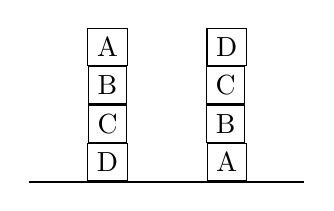
\begin{tikzpicture}[node distance = 0mm, block/.style args = {#1,#2}{fill=#1,text width=#2,shape=square}]
\node (initD) [draw]{D};
\node (initC) [draw, above=of initD.north]{C};
\node (initB) [draw, above=of initC.north]{B};
\node (initA) [draw, above=of initB.north]{A};
\draw[thick] (-1,-0.25) -- (2.5,-0.25);

\node (goalA) [draw, right=10mm of initD]{A};
\node (goalB) [draw, right=10mm of initC]{B};
\node (goalC) [draw, right=10mm of initB]{C};
\node (goalD) [draw, right=10mm of initA]{D};
\end{tikzpicture}
\vspace{0.6cm}
\end{subfigure}%
 \caption{\small Example of a task for learning a \strips\ action model in the blocksworld from a labeled plan.}
\label{fig:lexample}
\end{figure}


\subsection{Learning from multiple plans}
The previous task define the learning of planning action models from a single plan execution. These definitions can be extended to the more general case where learning from multiple plans:
\begin{itemize}
\item $\Lambda=\tup{\mathcal{M},\Psi,\Sigma}$ where $\Sigma=\{\sigma_1,\ldots,\sigma_{\tau}\}$ is a set of $(initial, final)$ state pairs, that we call {\em labels}. Each label $\sigma_t=(s_0^t,s_{n}^t)$, {\tt\small $1\leq t\leq \tau$}, comprises the {\em final} state $s_{n}^t$ resulting from executing an unknown plan $\pi_t=\tup{a_1^t, \ldots, a_n^t}$ starting from the {\em initial} state $s_0^t$.
\item $\Lambda=\tup{\mathcal{M},\Psi,\Sigma,\Pi}$ where $\Pi=\{\pi_1,\ldots,\pi_{\tau}\}$ is a given set of example plans where each plan $\pi_t=\tup{a_1^t, \ldots, a_n^t}$, {\small $1\leq t\leq \tau$}, is an action sequence that induces the corresponding state sequence $\tup{s_0^t, s_1^t, \ldots, s_n^t}$ such that, for each {\small $1\leq i\leq n$}, $a_i^t$ is applicable in $s_{i-1}^t$ and generates $s_i^t=\theta(s_{i-1}^t,a_i^t)$. 
\end{itemize}  



\section{Learning \strips\ action models with classical planning}
\label{sec:Section5}
Our approach for addressing a $\Lambda$ learning task is compiling it into a classical planning task $P_{\Lambda}$ with conditional effects. A planning compilation is a suitable approach for addressing $\Lambda$ because a solution must not only determine the \strips\ action model $\mathcal{M}'$ but also, the {\em unobserved} plan $\pi=\tup{a_1, \ldots, a_n}$, that explains the inputs to the lerning task. The intuition behind the compilation is that a solution to the resulting classical planning task is a sequence of actions that:

\begin{enumerate}
\item {\bf Programs the action model $\mathcal{M}'$}. A solution plan starts with a {\em prefix} that, for each $\xi\in\mathcal{M}$, determines which fluents $f\in F_v(\xi)$ belong to its $pre(\xi)$, $del(\xi)$ and $add(\xi)$ sets.
\item {\bf Validates the action model $\mathcal{M}'$ in $\mathcal{O}$}. The solution plan continues with a postfix that reproduces the given input knowledge using the programmed action model $\mathcal{M}'$.
\end{enumerate}


\subsection{Learning from state observations}
Given a learning task $\Lambda=\tup{\mathcal{M},\Psi,\mathcal{O}}$ the compilation outputs a classical planning task $P_{\Lambda}=\tup{F_{\Lambda},A_{\Lambda},I_{\Lambda},G_{\Lambda}}$:
\begin{itemize}
\item $F_{\Lambda}$ contains:
\begin{itemize}
\item The set of fluents $F$ built instantiating the predicates $\Psi$ with the objects appearing in the input observations $\mathcal{O}$, i.e. {\tt\small block1} and {\tt\small block2} in Figure~\ref{fig:lexample}.
\item Fluents $pre_f(\xi)$, $del_f(\xi)$ and $add_f(\xi)$, for every $f\in F_v(\xi)$, that represent the programmed action model. If a fluent $pre_f(\xi)/del_f(\xi)/add_f(\xi)$ holds, it means that $f$ is a precondition/negative/positive effect in the schema $\xi\in \mathcal{M}'$. For instance, the preconditions of the $stack$ schema (Figure~\ref{fig:stack}) are represented by the pair of fluents {\small\tt pre\_holding\_stack\_$v_1$} and {\small\tt pre\_clear\_stack\_$v_2$} set to {\em True}.
\item The fluents $mode_{prog}$ and $mode_{val}$ indicating whether the operator schemas are programmed or validated and the fluents $\{test_i\}_{1\leq i\leq n}$, indicating the observation where the action model is validated.
\end{itemize}
\item $I_{\Lambda}$ contains the fluents from $F$ that encode $s_0$ (the first observation) and $mode_{prog}$ set to true. Our compilation assumes that initially, operator schemas are programmed with every possible precondition (the most specific learning hypothesis), no negative effect and no positive effect. Therefore fluents $pre_f(\xi)$, for every $f\in F_v(\xi)$, hold also at the initial state.
\item $G_{\Lambda}=\bigcup_{1\leq i\leq n}\{test_i\}$, requires that the programmed action model is validated in all the input observations.
\item $A_{\Lambda}$ comprises three kinds of actions:
\begin{enumerate}
\item Actions for {\em programming} operator schema $\xi\in\mathcal{M}$:
\begin{itemize}
\item Actions for {\bf removing} a {\em precondition} $f\in F_v(\xi)$ from the action schema $\xi\in\mathcal{M}$.

\begin{small}
\begin{align*}
\hspace*{7pt}\pre(\mathsf{programPre_{f,\xi}})=&\{\neg del_{f}(\xi),\neg add_{f}(\xi),\\
& mode_{prog}, pre_{f}(\xi)\},\\
\cond(\mathsf{programPre_{f,\xi}})=&\{\emptyset\}\rhd\{\neg pre_{f}(\xi)\}.
\end{align*}
\end{small}

\item Actions for {\bf adding} a {\em negative} or {\em positive} effect $f\in F_v(\xi)$ to the action schema $\xi\in\mathcal{M}$.

\begin{small}
\begin{align*}
\hspace*{7pt}\pre(\mathsf{programEff_{f,\xi}})=&\{\neg del_{f}(\xi),\neg add_{f}(\xi),\\
& mode_{prog}\},\\
\cond(\mathsf{programEff_{f,\xi}})=&\{pre_{f}(\xi)\}\rhd\{del_{f}(\xi)\},\\
&\{\neg pre_{f}(\xi)\}\rhd\{add_{f}(\xi)\}.
\end{align*}
\end{small}
\end{itemize}

\item Actions for {\em applying} a programmed operator schema $\xi\in\mathcal{M}$ bound with objects $\omega\subseteq\Omega^{ar(\xi)}$. Given that the operators headers are known, the variables $pars(\xi)$ are bound to the objects in $\omega$ that appear at the same position.
\begin{small}
\begin{align*}
\hspace*{7pt}\pre(\mathsf{apply_{\xi,\omega}})=&\{pre_{f}(\xi)\implies p(\omega)\}_{\forall p\in\Psi,f=p(pars(\xi))}\\
&\cup \{\neg mode_{val}\},\\
\cond(\mathsf{apply_{\xi,\omega}})=&\{del_{f}(\xi)\}\rhd\{\neg p(\omega)\}_{\forall p\in\Psi,f=p(pars(\xi))},\\
&\{add_{f}(\xi)\}\rhd\{p(\omega)\}_{\forall p\in\Psi,f=p(pars(\xi))},\\
&\{mode_{prog}\}\rhd\{\neg mode_{prog}\},\\
&\{\emptyset\}\rhd\{mode_{val}\}.
\end{align*}
\end{small}

\item Actions for {\em validating} an observation {\tt\small $1\leq i\leq n$}.
\begin{small}
\begin{align*}
\hspace*{7pt}\pre(\mathsf{validate_{i}})=&s_i\cup\{test_j\}_{j\in 1\leq j<i}\\
&\cup\{\neg test_j\}_{j\in i\leq j\leq n}\cup \{mode_{val}\},\\
\cond(\mathsf{validate_{i}})=&\{\emptyset\}\rhd\{test_i,\neg mode_{val}\}.
\end{align*}
\end{small}
\end{enumerate}
\end{itemize}


\subsubsection{Compilation properties}

\begin{mylemma}
Soundness. Any classical plan $\pi$ that solves $P_{\Lambda}$ induces an action model $\mathcal{M}'$ that solves $\Lambda=\tup{\mathcal{M},\Psi,\mathcal{O}}$.
\end{mylemma}

\begin{proof}[Proof sketch]
\begin{small}
Once operator schemas $\mathcal{M}'$ are programmed, they can only be applied and validated, because of the $mode_{prog}$ fluent. In addition, $P_{\Lambda}$ is only solvable if fluents $\{test_i\}$, {\small $1\leq i\leq n$} hold at the last reached state. These goals can only be achieved executing an applicable sequence of programmed operator schemas that reaches every state $s_i\in\mathcal{O}$, starting from $s_0$ and following the sequence {\small $1\leq i\leq n$}. This means that the programmed action model $\mathcal{M}'$ complies with the provided observations $\mathcal{O}$ and hence, solves $\Lambda$.
\end{small}
\end{proof}


\begin{mylemma}
Completeness. Any \strips\ action model $\mathcal{M}'$ that solves a $\Lambda=\tup{\mathcal{M},\Psi,\mathcal{O}}$ learning task, is computable solving the corresponding classical planning task $P_{\Lambda}$.
\end{mylemma}

\begin{proof}[Proof sketch]
\begin{small}
By definition, $F_v(\xi)\subseteq F_\Lambda$ fully captures the full set of elements that can appear in a \strips\ action schema $\xi\in\mathcal{M}$ given its header and the set of predicates $\Psi$. The compilation does not discard any possible \strips\ action schema definable within $F_v$ that satisfies the state trajectory constraint given by $\mathcal{O}$.
\end{small}
\end{proof}

The size of the classical planning task $P_{\Lambda}$ output by the compilation depends on:
\begin{itemize}
\item The arity of the actions headers in $\mathcal{M}$ and the predicates $\Psi$ that are given as input to the $\Lambda$ learning task. The larger these numbers, the larger the $F_v(\xi)$ sets, that define the $pre_f(\xi)/del_f(\xi)/add_f(\xi)$ fluents set and the corresponding set of {\em programming} actions.
\item The number of given state observations. The larger $|\mathcal{O}|$, the more $test_i$ fluents and $\mathsf{validate_{i}}$ actions in $P_{\Lambda}$.
\end{itemize}

\subsection{Learning from a labeled plan}
We extend the compilation to consider labeled plans. Given a learning task $\Lambda=\tup{\mathcal{M},\Psi,\sigma,\pi}$, the compilation outputs a classical planning task $P_{\Lambda'}=\tup{F_{\Lambda'},A_{\Lambda'},I_{\Lambda'},G_{\Lambda'}}$:
\begin{itemize}
\item $F_{\Lambda'}$ extends $F_{\Lambda}$ with $F_{\Pi}=\{plan(name(\xi),\Omega^{ar(\xi)},j)\}$, the fluents to code the steps of the plans in $\Pi$, where $F_{\pi_t}\subseteq F_{\Pi}$ encodes $\pi_t\in \Pi$. Fluents $at_j$ and $next_{j,j+1}$, {\small $1\leq j< n$}, are also added to represent the current plan step and to iterate through the steps of a plan.
\item $I_{\Lambda'}$ extends $I_{\Lambda}$ with fluents $F_{\pi_1}$ plus fluents $at_1$ and $\{next_{j,j+1}\}$, {\small $1\leq j<n$}, for indicating the plan step where the action model is validated. Goals are $G_{\Lambda'}=G_{\Lambda}=\bigcup_{1\leq t\leq \tau}\{test_t\}$, as in the original compilation.
\item With respect to $A_{\Lambda'}$.
\begin{enumerate}
\item The actions for {\em programming} the preconditions/effects of a given operator schema $\xi\in\Xi$ are the same.
\item The actions for {\em applying} an already programmed operator have an extra precondition $f\in F_{\Pi}$, that encodes the current plan step, and extra conditional effects $\{at_{j}\}\rhd\{\neg at_{j},at_{j+1}\}_{\forall j\in [1,n]}$ for advancing to the next plan step. This mechanism forces that these actions are only applied as in the example plans.
\item The actions for {\em validating} the current learning example have an extra precondition, $at_{|\pi_t|}$, to indicate that the current plan $\pi_t$ was fully executed and extra conditional effects to unload plan $\pi_{t}$ and load the next plan $\pi_{t+1}$:
\begin{small}
\begin{align*}
&\{\emptyset\}\rhd\{\neg at_{|\pi_t|},at_1\}, \{f\}\rhd\{\neg f\}_{f\in F_{\pi_t}}, \{\emptyset\}\rhd\{f\}_{f\in F_{\pi_t+1}}.
\end{align*}
\end{small}
\end{enumerate}
\end{itemize}

\subsection{Partially specified action models}
Known preconditions and effects are encoded as fluents $pre_f(\xi)$, $del_f(\xi)$ and $add_f(\xi)$ set to true at the initial state $I_{\Lambda'}$. The corresponding programming actions, $\mathsf{programPre_{f,\xi}}$ and $\mathsf{programEff_{f,\xi}}$, become unnecessary and are removed from $A_{\Lambda'}$ making the classical planning task $P_{\Lambda'}$ easier to be solved.

To illustrate this, the classical plan of Figure~\ref{fig:plan} is a solution to a learning task $\Lambda''=\tup{\Psi,\Sigma,\Pi,\Xi_0}$ for getting the {\em blocksworld} action model where operator schemes for {\tt\small pickup}, {\tt\small putdown} and {\tt\small unstack} are specified in $\Xi_0$. This plan programs and validates the operator schema {\tt\small stack} from {\em blocksworld}, using the plan $\pi_1$ and label $\sigma_1$ shown in Figure~\ref{fig:lexample}. Plan steps $[0,8]$ program the preconditions of the {\tt\small stack} operator, steps $[9,13]$ program the operator effects and steps $[14,22]$ validate the programmed operators following the plan $\pi_1$ shown in the Figure~\ref{fig:lexample}.

In the extreme, when a fully specified \strips\ action model $\Xi$ is given in $\Xi_0$, the compilation validates whether an observed plan follows the given model. In this case, if a solution plan is found to $P_{\Lambda'}$, it means that the given \strips\ action model is {\em valid} for the given examples. If $P_{\Lambda'}$ is unsolvable it means that the given \strips\ action model is invalid since it is not compliant with all the given examples. Tools for plan validation like VAL~\cite{howey2004val} could also be used at this point.

\begin{figure}[hbt!]
{\footnotesize\tt
     {\bf 00} : (program\_pre\_clear\_stack\_v1)\\
     01 : (program\_pre\_handempty\_stack)\\
     02 : (program\_pre\_holding\_stack\_v2)\\
     03 : (program\_pre\_on\_stack\_v1\_v1)\\
     04 : (program\_pre\_on\_stack\_v1\_v2)\\
     05 : (program\_pre\_on\_stack\_v2\_v1)\\
     06 : (program\_pre\_on\_stack\_v2\_v2)\\
     07 : (program\_pre\_ontable\_stack\_v1)\\
     08 : (program\_pre\_ontable\_stack\_v2)\\
     {\bf 09} : (program\_eff\_clear\_stack\_v1)\\
    10 : (program\_eff\_clear\_stack\_v2)\\
    11 : (program\_eff\_handempty\_stack)\\
    12 : (program\_eff\_holding\_stack\_v1)\\
    13 : (program\_eff\_on\_stack\_v1\_v2)\\
    {\bf 14} : (apply\_unstack a b i1 i2)\\
    15 : (apply\_putdown a i2 i3)\\
    16 : (apply\_unstack b c i3 i4)\\
    17 : (apply\_stack b a i4 i5)\\
    18 : (apply\_unstack c d i5 i6)\\
    19 : (apply\_stack c b i6 i7)\\
    20 : (apply\_pickup d i7 i8)\\
    21 : (apply\_stack d c i8 i9)\\
    {\bf 22} : (validate\_1)
}
 \caption{\small Plan for programming and validating the $stack$ schema using plan $\pi_1$ and label $\sigma_1$ (shown in Figure~\ref{fig:lexample}) as well as previously specified operator schemes for $pickup$, $putdown$ and $unstack$.}
\label{fig:plan}
\end{figure}

\subsection{Static predicates}
A {\em static predicate} $p \in \Psi$ is a predicate that does not appear in the effects of any action~\cite{fox:TIM:JAIR1998}. Therefore, one can get rid of the mechanism for programming these predicates in the effects of any action schema while keeping the compilation complete. Given a static predicate $p$:
\begin{itemize}
\item Fluents $del_f(\xi)$ and $add_f(\xi)$, such that $f\in F_v$ is an instantiation of the static predicate $p$ in the set of {\em variable objects} $\Omega_v$, can be discarded for every $\xi\in\Xi$.
\item Actions $\mathsf{programEff_{f,\xi}}$ (s.t. $f\in F_v$ is an instantiation of $p$ in $\Omega_v$) can also be discarded for every $\xi\in\Xi$.
\end{itemize}

Static predicates can also constrain the space of possible preconditions by looking at the given set of labels $\Sigma$. One can assume that if a precondition $f\in F_v$ (s.t. $f\in F_v$ is an instantiation of a static predicate in $\Omega_v$) is not compliant with the labels in $\Sigma$ then, fluents $pre_f(\xi)$ and actions $\mathsf{programPre_{f,\xi}}$ can be discarded for every $\xi\in\Xi$. For instance in the {\em zenotravel} domain $pre\_next\_board\_v1\_v1$, $pre\_next\_debark\_v1\_v1$, $pre\_next\_fly\_v1\_v1$, $pre\_next\_zoom\_v1\_v1$, $pre\_next\_refuel\_v1\_v1$ can be discarded (and their corresponding programming actions) because a precondition {\tt\small(next ?v1 ?v1 - flevel)} will never hold at any state in $\Sigma$.

Looking at the given example plans, fluents $pre_f(\xi)$ and actions $\mathsf{programPre_{f,\xi}}$ are discardable for every $\xi\in\Xi$ if a precondition $f\in F_v$ (s.t. $f\in F_v$ is an instantiation of a static predicate in $\Omega_v$) is not possible according to $\Pi$. Back to the {\em zenotravel} domain, if an example plan $\pi_t\in \Pi$ contains the action {\tt\small (fly plane1 city2 city0 fl3 fl2)} and the corresponding label $\sigma_t\in\Sigma$ contains the static literal {\tt\small (next fl2 fl3)} but does not contain {\tt\small (next fl2 fl2)}, {\tt\small (next fl3 fl3)} or {\tt\small (next fl3 fl2)} the only possible precondition including the static predicate is $pre\_next\_fly\_v5\_v4$.

\subsection{Learning from multiple plans}
The $\Lambda=\tup{\mathcal{M},\Psi,\Sigma}$ can be solved with the previous compilation $P_{\Lambda}$. On the other hand, the learning task $\Lambda=\tup{\mathcal{M},\Psi,\Sigma,\Pi}$ requires modifying the previous compilation. In particular, the actions for {\em validating} the labeled plan $\pi_t\in\Pi$ with the corresponding label $\sigma_t\in\Sigma$, {\tt\small $1\leq t\leq \tau$}.
\begin{small}
\begin{align*}
\hspace*{7pt}\pre(\mathsf{validate_{t}})=&G_t\cup\{test_j\}_{j\in 1\leq j<t}\\
&\cup\{\neg test_j\}_{j\in t\leq j\leq \tau}\cup \{\neg mode_{prog}\},\\
\cond(\mathsf{validate_{t}})=&\{\emptyset\}\rhd\{test_t\}.
\end{align*}
\end{small}


\section{Evaluating \strips\ action models}
\label{sec:Section6}
We assess how well a \strips\ action model $\mathcal{M}$ explains a given sequence of observations $\mathcal{O}$ according to the amount of {\em edition} required by $\mathcal{M}$ to induce $\mathcal{O}$. %In the extreme, if $\mathcal{M}$ perfectly explains $\mathcal{O}$, no model {\em edition} is necessary.

\subsection{Edition of \strips\ action models}

We first define the allowed \emph{operations} to edit a given \strips\ action model. With the aim of keeping a tractable branching factor of the planning instances that results from our compilation, we only define two {\em edit operations}:
\begin{itemize}
\item {\em Deletion}. A fluent $pre_f(\xi)/del_f(\xi)/add_f(\xi)$ is removed from the operator schema $\xi\in\mathcal{M}$, $f\in F_v(\xi)$.
\item {\em Insertion}. A fluent $pre_f(\xi)/del_f(\xi)/add_f(\xi)$ is added to the operator schema $\xi\in\mathcal{M}$, $f\in F_v(\xi)$.
\end{itemize}

We can now formalize an edit distance that quantifies how dissimilar two given \strips\ action models are. The distance is symmetric and meets the {\em metric axioms} provided that the two {\em edit operations} have the same positive cost.

\begin{mydefinition}
Let $\mathcal{M}$ and $\mathcal{M}'$ be two \strips\ action models, both built from the same set of possible elements $F_v$. The {\bf edit distance}, denoted as $\delta(\mathcal{M},\mathcal{M}')$, is the minimum number of {\em edit operations} required to transform $\mathcal{M}$ into $\mathcal{M}'$.
\end{mydefinition}

Since $F_v$ is a bound set, the maximum number of edits that can be introduced to a given action model defined within $F_v$ is bound as well. In more detail, for an operator schema $\xi\in\mathcal{M}$ the maximum number of edits that can be introduced to their precondition set is $|F_v(\xi)|$ while the max number of edits that can be introduced to the effects is twice $|F_v(\xi)|$.

\begin{mydefinition}
The \textbf{maximum edit distance} of an \strips\ action model $\mathcal{M}$ built from the set of possible elements $F_v$ is $\delta(\mathcal{M},*)=\sum_{\xi\in\mathcal{M}} 3|F_v(\xi)|$.
\end{mydefinition}


\subsection{The \strips\ edit distance}

We define now an edit distance to asses the quality of a learned action model with respect to a sequence of state observations.

\begin{mydefinition}
Given an action model $\mathcal{M}$, built from $F_v$, and the observations sequence $\mathcal{O}=\tup{s_0, s_1, \ldots, s_n}$. The {\bf observation edit distance}, denoted by  $\delta(\mathcal{M},\mathcal{O})$, is the minimal edit distance from $\mathcal{M}$ to any model $\mathcal{M}'$, defined also within $F_v$, such that $\mathcal{M}'$ can produce a plan $\pi=\tup{a_1, \ldots, a_n}$ that induces $\mathcal{O}$; \[\delta(\mathcal{M},\mathcal{O})=\min_{\forall \mathcal{M}' \rightarrow \mathcal{O}} \delta(\mathcal{M},\mathcal{M}')\]
\end{mydefinition}

The $\Lambda$ learning tasks can swap the roles of two operators whose headers match or two action parameters that belong to the same type (e.g. the {\em blocksworld} operator {\small\tt stack} can be {\em learned} with the preconditions and effects of the {\small\tt unstack} operator and vice versa, or the parameters of the {\small\tt stack} operator can be swapped). The {\em observation edit distance} is a semantic measure that is robust to role changes of this kind.

Unlike the error function defined by {\sc ARMS}~\cite{yang2007learning}, the {\em observation edit distance} assesses, with a single expression, the flaws in the preconditions and effects of a given learned model. This fact enables the recognition of \strips\ action models. The idea, taken from {\em plan recognition as planning}~\cite{ramirez2009plan}, is to map distances into likelihoods. The {\em observation edit distance} could be mapped into a likelihood with the following expression $P(\mathcal{O}|\mathcal{M})=1-\frac{\delta(\mathcal{M},\mathcal{O})}{\delta(\mathcal{M},*)}$.


The edit distance can also be defined with respect to a labeled plan. 

\begin{mydefinition}
  Given an action model $\mathcal{M}$, built from $F_v$, and the plan $\pi=\tup{a_1, \ldots, a_n}$  with the corresponding label $\sigma=(s_0,s_{n})$. The {\bf plan edit distance}, denoted by  $\delta(\mathcal{M},\mathcal{\pi},\mathcal{\sigma})$, is the minimal edit distance from $\mathcal{M}$ to any model $\mathcal{M}'$, defined also within $F_v$, such that $\mathcal{M}'$ can produce a plan $\pi$ that induces $\sigma$; \[\delta(\mathcal{M},\mathcal{O})=\min_{\forall \mathcal{M}' \rightarrow \mathcal{\sigma}} \delta(\mathcal{M},\mathcal{M}')\]
\end{mydefinition}

Last but not least, the edit distance can also be defined with respect to multiple plans. 

\subsection{Computing the edit distance}

Our compilation is extensible to compute the {\em edit distance} between two models. A solution to the planning task resulting from the extended compilation is a sequence of actions that edits the action model $\mathcal{M}$ to  produce $\mathcal{M}'$ using to the two {\em edit operations}.

The output of the extended compilation is a classical planning task $P_{\Lambda}'=\tup{F_{\Lambda},A_{\Lambda}',I_{\Lambda}',G_{\Lambda}}$:

\begin{itemize}
\item $F_{\Lambda}$ and $G_{\Lambda}$ are defined as in the previous compilation.
\item $I_{\Lambda}'$ contains the fluents from $F$ that encode $s_0$ and $mode_{prog}$ set to true. In addition, the input action model $\mathcal{M}$ is now encoded in the initial state. This means that the fluents $pre_f(\xi)/del_f(\xi)/add_f(\xi)$, $f\in F_v(\xi)$, hold in the initial state iff they appear in $\mathcal{M}$.
\item $A_{\Lambda}'$, comprises the same three kinds of actions of $A_{\Lambda}$. The actions for {\em applying} an already programmed operator schema and the actions for {\em validating} an observation are defined exactly as in the previous compilation. The only difference here is that the actions for {\em programming} the operator schema now implement the two {\em edit operations} (i.e. include actions for {\em inserting} a precondition and for {\em deleting} a negative/positive effect).
\end{itemize}

To illustrate this, the plan of Figure~\ref{fig:plan} solves the classical planning task $P_{\Lambda}'$ that corresponds to editing a \emph{blocksworld} action model where the positive effects {\tt\small (handempty)} and {\tt\small (clear ?v1)} of the {\tt\small stack} schema are missing. The plan edits first the {\tt\small stack} schema, {\em inserting} these two positive effects, and then validates the edited action model in the five-observation sequence of Figure~\ref{fig:lexample}.

Our interest when computing the {\em observation edit distance} is not in $\mathcal{M}'$ but in the number of required {\em edit operations}, e.g. $\delta(\mathcal{M},\mathcal{O})=2$ for the example in Figure~\ref{fig:plan-edistance}. The {\em observation edit distance} is exactly computed if $P_{\Lambda}'$ is optimally solved (according to the number of edit actions); is approximated if $P_{\Lambda}'$ is solved with a satisfying planner (our case); and is a less accurate estimate (but faster to be computed) if the solved task is a relaxation of $P_{\Lambda}'$~\cite{bonet2001planning}.

\begin{figure}[hbt!]
{\tt\small
00 : (insert\_add\_handempty\_stack)\\
01 : (insert\_add\_clear\_stack\_var1)
}
 \caption{\small Plan for editing a given {\em blockswold} schema and validating it at the state observations shown in Figure~\ref{fig:lexample}.}
\label{fig:plan-edistance}
\end{figure}


\subsection{Computing the observations distance}

Our compilation is extensible to compute the {\em observation edit distance} by simply considering that the model $\mathcal{M}$, given in $\Lambda=\tup{\mathcal{M},\Psi,\mathcal{O}}$, is {\em non-empty}. In other words, now $\mathcal{M}$ is a set of given operator schemas, wherein each $\xi\in\mathcal{M}$ initially contains $head(\xi)$ but also the $pre(\xi)$, $del(\xi)$ and $add(\xi)$ sets. A solution to the planning task resulting from the extended compilation is a sequence of actions that:

\begin{enumerate}
\item {\bf Edits the action model $\mathcal{M}$}. A solution plan starts with a {\em prefix} that modifies the preconditions and effects of the action schemas in $\mathcal{M}$ using to the two {\em edit operations}.
\item {\bf Validates the edited model $\mathcal{M}'$ in $\mathcal{O}$}. The solution plan continues with a postfix that validates the edited model on the given observations $\mathcal{O}$, as in Section~\ref{sec:Section4}.
\end{enumerate}

Now $\Lambda$ is not a learning task but the task of editing $\mathcal{M}$ to produce the observations $\mathcal{O}$, which results in the edited model $\mathcal{M}'$. The output of the extended compilation is a classical planning task $P_{\Lambda}'=\tup{F_{\Lambda},A_{\Lambda}',I_{\Lambda}',G_{\Lambda}}$:

\begin{itemize}
\item $F_{\Lambda}$ and $G_{\Lambda}$ are defined as in the previous compilation.
\item $I_{\Lambda}'$ contains the fluents from $F$ that encode $s_0$ and $mode_{prog}$ set to true. In addition, the input action model $\mathcal{M}$ is now encoded in the initial state. This means that the fluents $pre_f(\xi)/del_f(\xi)/add_f(\xi)$, $f\in F_v(\xi)$, hold in the initial state iff they appear in $\mathcal{M}$.
\item $A_{\Lambda}'$, comprises the same three kinds of actions of $A_{\Lambda}$. The actions for {\em applying} an already programmed operator schema and the actions for {\em validating} an observation are defined exactly as in the previous compilation. The only difference here is that the actions for {\em programming} the operator schema now implement the two {\em edit operations} (i.e. include actions for {\em inserting} a precondition and for {\em deleting} a negative/positive effect).
\end{itemize}

To illustrate this, the plan of Figure~\ref{fig:plan} solves the classical planning task $P_{\Lambda}'$ that corresponds to editing a \emph{blocksworld} action model where the positive effects {\tt\small (handempty)} and {\tt\small (clear ?v1)} of the {\tt\small stack} schema are missing. The plan edits first the {\tt\small stack} schema, {\em inserting} these two positive effects, and then validates the edited action model in the five-observation sequence of Figure~\ref{fig:lexample}.

Our interest when computing the {\em observation edit distance} is not in $\mathcal{M}'$ but in the number of required {\em edit operations} for that $\mathcal{M}'$ is validated in the given observations, e.g. $\delta(\mathcal{M},\mathcal{O})=2$ for the example in Figure~\ref{fig:plan-odistance}. The {\em observation edit distance} is exactly computed if $P_{\Lambda}'$ is optimally solved (according to the number of edit actions); is approximated if $P_{\Lambda}'$ is solved with a satisfying planner (our case); and is a less accurate estimate (but faster to be computed) if the solved task is a relaxation of $P_{\Lambda}'$~\cite{bonet2001planning}.

\begin{figure}[hbt!]
{\tt\small
00 : (insert\_add\_handempty\_stack)\\
01 : (insert\_add\_clear\_stack\_var1)\\
02 : (apply\_unstack block2 block1)\\
03 : (validate\_1)\\
04 : (apply\_putdown block2)\\
05 : (validate\_2)\\
06 : (apply\_pickup block1)\\
07 : (validate\_3)\\
08 : (apply\_stack block1 block2)\\
09 : (validate\_4)\\
}
 \caption{\small Plan for editing a given {\em blockswold} schema and validating it at the state observations shown in Figure~\ref{fig:lexample}.}
\label{fig:plan-odistance}
\end{figure}



\section{Recognition of \strips\ action models}
\label{sec:Section7}



\section{Evaluation}
\label{sec:Section8}
This section evaluates the performance of our approach for learning \strips\ action models starting from different amounts of available input knowledge.

\subsection{Setup}
The domains used in the evaluation are IPC domains that satisfy the \strips\ requirement~\cite{fox2003pddl2}, taken from the {\sc planning.domains} repository~\cite{muise2016planning}. We only use 5 learning examples for each domain and they are fixed for all the experiments so we can evaluate the impact of the input knowledge in the quality of the learned models. All experiments are run on an Intel Core i5 3.10 GHz x 4 with 4 GB of RAM.
\begin{itemize}
\item {\bf Reproducibility}. We make fully available the compilation source code, the evaluation scripts and the used benchmarks at this anonymous repository {\em https://github.com/anonsub/strips-learning} so any experimental data reported in the paper is fully reproducible. 
\item {\bf Planner}. The classical planner we use to solve the instances that result from our compilations is {\sc Madagascar}~\cite{rintanen2014madagascar}. We use {\sc Madagascar} because its ability to deal with planning instances populated with dead-ends. In addition, SAT-based planners can apply the actions for programming preconditions in a single planning step (in parallel) because these actions do not interact. Actions for programming action effects can also be applied in a single planning step reducing significantly the planning horizon.
\item {\bf Metrics}.The quality of the learned models is quantified with the {\em precision} and {\em recall} metrics. These two metrics are frequently used in {\em pattern recognition}, {\em information retrieval} and {\em binary classification} and are more informative that simply counting the number of errors in the learned model or computing the {\em symmetric difference} between the learned and the reference model~\cite{davis2006relationship}. Intuitively, precision gives a notion of {\em soundness} while recall gives a notion of the {\em completeness} of the learned models. Formally, $Precision=\frac{tp}{tp+fp}$, where $tp$ is the number of true positives (predicates that correctly appear in the action model) and $fp$ is the number of false positives (predicates appear in the learned action model that should not appear). Recall is formally defined as $Recall=\frac{tp}{tp+fn}$ where $fn$ is the number of false negatives (predicates that should appear in the learned action model but are missing).
\end{itemize}
  
\section{Conclussions}
\label{sec:Section9}



\begin{small}
\subsection*{Acknowledgment}
This work is supported by the Spanish MINECO project TIN2017-88476-C2-1-R. Diego Aineto is partially supported by the {\it FPU16/03184} and Sergio Jim\'enez by the {\it RYC15/18009}, both programs funded by the Spanish government.
\end{small}


%% References
%%
%% Following citation commands can be used in the body text:
%% Usage of \cite is as follows:
%%   \cite{key}         ==>>  [#]
%%   \cite[chap. 2]{key} ==>> [#, chap. 2]
%%

%% References with BibTeX database:

\bibliographystyle{elsarticle-num}
\bibliography{planlearnbibliography.bib}

%% Authors are advised to use a BibTeX database file for their reference list.
%% The provided style file elsarticle-num.bst formats references in the required Procedia style

%% For references without a BibTeX database:

% \begin{thebibliography}{00}

%% \bibitem must have the following form:
%%   \bibitem{key}...
%%

% \bibitem{}

% \end{thebibliography}



\end{document}

%%
%% End of file `ecrc-template.tex'. 
